\documentclass{beamer}
%\documentclass[xcolor={dvipsnames,table}]{beamer}
%\usetheme{Warsaw}
%\usetheme{AnnArbor}
%\usetheme{Frankfurt}
\usetheme{Madrid}
%\setbeamertemplate{title page}[default][colsep=-0bp,rounded=false]
%\setbeamertemplate{frametitle}[default][colsep=-4bp,rounded=false,shadow=false]
%\setbeamertemplate{blocks}[rounded][shadow=false]


\title{PSET5: Ordered Collections \\ Priority Queues}


\date{March 17, 2023}

\author{Anusha Murali}


\usepackage{tikz-qtree}
\begin{document}

%\frame{\titlepage}

\begin{frame}[fragile]
\titlepage

\end{frame}


\begin{frame}[fragile]
\frametitle{Tasks to do}

\begin{block}{Part II: Implement Ordered Collections with Priority Queues}
\begin{enumerate}
\item Complete \textcolor{red}{ListQueue}: elements are stored a list
\item Complete \textcolor{red}{TreeQueue}: elements are stored in a BST
\item Complete \textcolor{red}{HeapQueue}: elements are stored in a balanced binary tree
\end{enumerate}
\end{block}
\end{frame}


\begin{frame}[fragile]

\vspace*{0.5in}

\centerline{\huge HeapQueue}

\vspace*{0.2in}
\begin{center}
Task: Use a Binary Heap to implement the signature of PRIOQUEUE .
\end{center}

\end{frame}





%%%%%%%%%%%%%%%%%%%%%%%
\begin{frame}[fragile]
\frametitle{Step 1 Load Files}

\begin{block}{Load Files}
\begin{enumerate}
\item \# \#use "order.ml"
\item \# \#use "orderedcoll.ml"
\item \# \#use "prioqueue.ml"
\end{enumerate}
\end{block}
\end{frame}


\frame[fragile]
\frametitle{Step 2: Complete the {\tt BinaryHeap} functor}


\begin{alertblock}{Complete get\_top}
\hspace*{1.0in}  let get\_top (t : tree) : elt =\\
\hspace*{1.15in}       failwith "BinaryHeap get\_top not implemented"
\end{alertblock}

\begin{block}{get\_top}
\begin{verbatim}
  let get_top (t : tree) : elt =
      match t with
      | Leaf e -> e
      | OneBranch (e, _) -> e
      | TwoBranch (_, e, _, _) -> e
\end{verbatim}
\end{block}

\end{frame}



\frame[fragile]
\frametitle{Step 2: Complete the {\tt BinaryHeap} functor}


\begin{alertblock}{Complete fix}
\hspace*{1.0in}let fix (t : tree) : tree =\\
\hspace*{1.15in}      failwith "BinaryHeap fix not implemented"
\end{alertblock}

\begin{block}{fix\_top: A helper function, which changes the top element of t with e}
\begin{verbatim}
 let fix_top (e : elt) (t : tree) : tree =
    match t with
    | Leaf _ -> Leaf e
    | OneBranch (_, e2) -> OneBranch(e, e2)
    | TwoBranch (x, _, t1, t2) -> TwoBranch(x, e, t1, t2)
\end{verbatim}
\end{block}

\end{frame}



\frame[fragile]
\frametitle{Step 2: Complete the {\tt BinaryHeap} functor}

{\tiny
\begin{block}{fix}
\begin{verbatim}
 let rec fix (t : tree) : tree =
      match t with
      | Leaf _ -> t
      | OneBranch(e1, e2) ->
        (match Elt.compare e1 e2 with
         | Less -> t
         | Equal
         | Greater -> OneBranch(e2, e1) )
      | TwoBranch(x, e, t1, t2) ->
        (* Get the top elements of t1 and t2 and determine which is smaller *)
        let (e1, e2) = (get_top t1, get_top t2) in
        (match Elt.compare e1 e2 with
         | Less
         | Equal ->  (match Elt.compare e e1 with
                      | Less -> t
                      | Equal
                      | Greater ->
                        TwoBranch(x, e1, fix (fix_top e t1), t2))
         | Greater -> (match Elt.compare e e2 with
                       | Less -> t
                       | Equal
                       | Greater -> TwoBranch(x, e2, t1, fix (fix_top e t2))))
\end{verbatim}
\end{block}
}

\end{frame}


\frame[fragile]
\frametitle{Step 2: Complete the {\tt BinaryHeap} functor}


\begin{alertblock}{Complete get\_last}
\hspace*{1.0in}let get\_last (t : tree) : elt * queue =\\
\hspace*{1.15in}      failwith "BinaryHeap get\_last not implemented"
\end{alertblock}

{\tiny
\begin{block}{get\_last}
\begin{verbatim}
 let rec get_last (t : tree) : elt * queue =
      match t with
      | Leaf e -> (e, Empty)
      | OneBranch (e1, e2) -> (e2, Tree (Leaf e1))
      | TwoBranch (even_or_odd, e, t1, t2) ->
        (match even_or_odd with
         | Odd -> (match t1 with
                   | Leaf last -> (last, Tree (OneBranch (e, get_top t2)))
                   | _ -> (fst (get_last t1),
                           Tree (TwoBranch
                                 (Even, e, (extract_tree (snd (get_last t1))),
                                            t2))))
         | Even -> (match t2 with
                   | Leaf last -> (last, Tree (OneBranch(e, get_top t1)))
                   | _ -> (fst (get_last t2),
                           Tree (TwoBranch
                                (Odd, e, t1,
                                           (extract_tree (snd (get_last t2))))))))
\end{verbatim}
\end{block}
}


\end{frame}












\begin{frame}{fragile}
\frametitle{Step 2: Complete the {\tt BinaryHeap} functor}

\begin{block}{Re-load prioqueue.ml (with your completed functions)}
\begin{enumerate}
\item \# \#use "prioqueue.ml"
\end{enumerate}
\end{block}

\begin{example}
Now the examples in the next slides should work
\end{example}
\end{frame}
      



\begin{frame}{fragile}
\frametitle{Test add function}

\begin{example}
\begin{enumerate}
\item First create an empty HeapQueue called myQ \\
        \# {\bf  let myQ = IntHeapQueue.empty;;}
\item Insert 65\\
 \# {\bf let myQ = IntHeapQueue.add 65 myQ};;
\end{enumerate}
\end{example}

\tikzset{every tree node/.style={minimum width=2.5em,draw,circle},
         blank/.style={draw=none},
         edge from parent/.style=
         {draw,edge from parent path={(\tikzparentnode) -- (\tikzchildnode)}},
         level distance=1.5cm, sibling distance=1.5cm}
\begin{center}
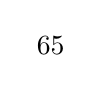
\begin{tikzpicture}
 \Tree [.65  ]
 \end{tikzpicture}
\end{center}

\begin{example}
Print the queue:\\

\# {\bf IntHeapQueue.to\_string myQ;;} \\

\hspace*{1in} \textcolor{red}{Output:} - : string = "Leaf 65"

\end{example}

\end{frame}


\begin{frame}{fragile}
\frametitle{Test add function}

\begin{example}
\begin{enumerate}
\item Now insert 40\\
 \# {\bf let myQ = IntHeapQueue.add 40 myQ};;
\end{enumerate}
\end{example}

\tikzset{every tree node/.style={minimum width=2.5em,draw,circle},
         blank/.style={draw=none},
         edge from parent/.style=
         {draw,edge from parent path={(\tikzparentnode) -- (\tikzchildnode)}},
         level distance=1.5cm, sibling distance=1.5cm}
\begin{center}
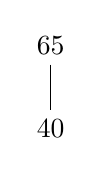
\begin{tikzpicture}
 \Tree [.65  [.40 ]   ]
\end{tikzpicture}
\end{center}


\begin{example}
Print the queue:\\

\# {\bf IntHeapQueue.to\_string myQ;;} \\

\hspace*{0.2in} \textcolor{red}{Output:} - : string = "OneBranch (40, 65)"

\end{example}

\end{frame}


\begin{frame}{fragile}
\frametitle{Test add function}

\begin{example}
\begin{enumerate}
\item Now insert 50\\
 \# {\bf let myQ = IntHeapQueue.add 50 myQ};;
\end{enumerate}
\end{example}

\tikzset{every tree node/.style={minimum width=2.5em,draw,circle},
         blank/.style={draw=none},
         edge from parent/.style=
         {draw,edge from parent path={(\tikzparentnode) -- (\tikzchildnode)}},
         level distance=1.5cm, sibling distance=1.5cm}
\begin{center}
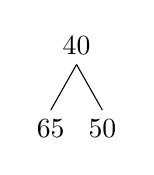
\begin{tikzpicture}
 \Tree [.40  [.65 ] [.50 ] ]  
\end{tikzpicture}
\end{center}

\begin{example}
Print the queue:\\

\# {\bf IntHeapQueue.to\_string myQ;;} \\

\hspace*{0.2in} \textcolor{red}{Output:} - : string = "TwoBranch (Even, 40, Leaf 65, Leaf 50)"

\end{example}

\end{frame}



\begin{frame}{fragile}
\frametitle{Test add function}

\begin{example}
\begin{enumerate}
\item Now insert 70\\
 \# {\bf let myQ = IntHeapQueue.add 70 myQ};;
\end{enumerate}
\end{example}

\tikzset{every tree node/.style={minimum width=2.5em,draw,circle},
         blank/.style={draw=none},
         edge from parent/.style=
         {draw,edge from parent path={(\tikzparentnode) -- (\tikzchildnode)}},
         level distance=1.5cm, sibling distance=1.5cm}
\begin{center}
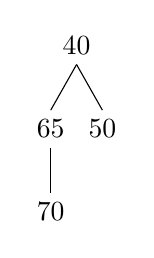
\begin{tikzpicture}
 \Tree [.40   [.65  [.70 ] ]    [.50 ] ]
\end{tikzpicture}
\end{center}

 "TwoBranch (Odd, 40, OneBranch (65, 70), Leaf 50)"


\end{frame}




\begin{frame}{fragile}
\frametitle{Test add function}

\begin{example}
\begin{enumerate}
\item Now insert 30\\
 \# {\bf let myQ = IntHeapQueue.add 30 myQ};;
\end{enumerate}
\end{example}

\tikzset{every tree node/.style={minimum width=2.5em,draw,circle},
         blank/.style={draw=none},
         edge from parent/.style=
         {draw,edge from parent path={(\tikzparentnode) -- (\tikzchildnode)}},
         level distance=1.5cm, sibling distance=1.5cm}
\begin{center}
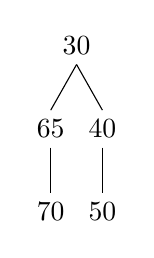
\begin{tikzpicture}
 \Tree [.30   [.65  [.70 ] ]   [.40  [.50 ] ] ]
\end{tikzpicture}
\end{center}
"TwoBranch (Even, 30, OneBranch (65, 70), OneBranch (40, 50))"
\end{frame}





%%%%%%%%%%%%%%%

\begin{frame}{fragile}
\frametitle{Test take function}

\begin{example}
\begin{enumerate}
\item The take function returns the element with the highest priority (i.e: smallest value) and the remaining queue\\
 \# {\bf let (hiPri, myQ) = IntHeapQueue.take myQ};;
\item The value of {\bf hiPri = 30} and the new {\bf myQ} is shown below
\end{enumerate}
\end{example}

\tikzset{every tree node/.style={minimum width=2.5em,draw,circle},
         blank/.style={draw=none},
         edge from parent/.style=
         {draw,edge from parent path={(\tikzparentnode) -- (\tikzchildnode)}},
         level distance=1.5cm, sibling distance=1.5cm}
\begin{center}
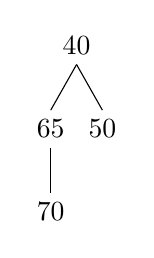
\begin{tikzpicture}
 \Tree [.40   [.65  [.70 ] ]    [.50 ] ]
\end{tikzpicture}
\end{center}

\end{frame}







\begin{frame}{fragile}
\frametitle{Important comment on HeapQueue}
\begin{block}{Average and worst-case time complexity}
\begin{enumerate}
\item The Heap Queue is always (almost) balanced. So, the height of the tree is $\log n$. Hence the  average time complexity and the worst-case time complexity to search an element are both equal to $O(\log n)$
\end{enumerate}
\end{block}

\end{frame}


\end{document}

